\documentclass[runningheads]{llncs}
\usepackage[latin1]{inputenc}
\usepackage[T1]{fontenc}
\usepackage[ngerman]{babel}
\usepackage{array}
\usepackage{wrapfig}
\usepackage{graphicx}
\usepackage{microtype}
\usepackage[bookmarks=true,
breaklinks=true,
colorlinks=true,
hyperindex=true,
linkcolor=black,
citecolor=black,
urlcolor=black]{hyperref}

%opening
\title{Die Entwicklungswerkzeuge SVN und Maven}
\author{Aleksandar Tolev}
\institute{Institute of Architecture of Application Systems, University of Stuttgart, Germany\\
          Universit�tsstrasse 38, 70569 Stuttgart, Germany\\
           \email{tolevar@studi.informatik.uni-stuttgart.de}}

\begin{document}

\maketitle

\begin{abstract}
 In dieser Ausarbeitung werden die zwei Werkzeuge, Subversion und Maven, behandelt. Sie werden in einem Softwareprojekt h�ufig zur Versionierung und zur vereinfachten Kompilierung eingesetzt.
\end{abstract}


\section{Einleitung}

Heutzutage sind Softwareprojekte im gr��eren Umfang keine Seltenheit mehr. Dabei ist es wichtig einen �berblick �ber die Dateien und ihre �nderungen zu haben. Das �bernimmt die Versionskontrolle Subversion. Mit ihrer Hilfe ist die M�glichkeit geboten stets mit der aktuellsten Version einer Datei zu arbeiten. Durch Subversion k�nnen mehrere Projektlinien des gleichen Hauptprojektes gleichzeitig verfolgt werden. Dabei entstehen keine Komplikationen innerhalb des Projektes. Im Fehlerfall k�nnen vorgenommene �nderungen zur�ckgenommen werden, indem man zu einer vorherigen Version zur�ckkehrt.

Durch das Arbeiten in gro�en Teams ist nicht immer eine gemeinsame Projektstruktur gegeben, da unterschiedliche Entwickler unterschiedliche Strukturen erstellen. Dadurch kann es zu nicht einheitlichen Ordnerstrukturen kommen, was zu unterschiedlichen Buidlfiles f�hrt. Mit Maven wird ein einheitliches Build-Tool bereitgestellt, welches den Entwicklern die M�glichkeit bietet, auf einem gemeinsamen Standard die Implementierung abzuarbeiten. 

Diese beiden Themen werden in Bezug auf das Studienprojekt 2008/2009 \glqq DecidR\grqq{} vorgestellt und sollen zudem den \glqq DecidR-Teammitgliedern\grqq{} vermittelt werden, damit diese ein Verst�ndnis f�r die beiden Werkzeuge Subversion und Maven bekommen. Diese Werkzeuge sollten nach M�glichkeit im Projekt angewendet werden. In Abschnitt 2 wird das Werkzeug \glqq Subversion\grqq{} vorgestellt. Daran schlie�t sich Abschnitt 3 an, in dem Maven beschrieben wird. Den Abschluss der Arbeit bildet die Zusammenfassung in Abschnitt 4.
\section{SVN/Subversion}
\subsection{Definition und Geschichte des SVN}
Der Begriff Subversion bzw. Subversion ist klar definiert. Der Begriff bezieht sich zum einen auf die politisch-soziologische Deutung der Subversion, die eine T�tigkeit im Verborgenen, deren Ziel der Umsturz einer bestehenden Ordnung durch Unterwanderung und Untergrabung ist, definiert. Desweiteren bezieht sich der Begriff auf die sub version, also Unterversion oder der fr�heren Version. Das bedeutet Subversion dient der Versionskontrolle. Mit SVN k�nnen verschiedene Entwickler an Dateien arbeiten. Dabei wird immer die aktuellste Version bereitgestellt, sodass alle Entwickler auf dem gleichen Stand sind. \\
Subversion wurde seit Anfang 2000 bei CollabNet entwickelt und erreichte Februar 2004 seine stabile Version 1.0. Seitdem wurden immer neuere Versionen entwickelt, die letzte ist die Version 1.5 (Juni 2008).Folgend werden die �nderungen in den einzelnen Versionen aufgelistet:
\begin{description}
 \item[Version 1.1] Repositories m�ssen nicht mehr in einer Berkley-Datenbank verwaltet werden, sondern man kann auch direkt das Dateisystem benutzen
 \item[Version 1.2] Die Sperrung von Dateien wurde eingef�hrt, was vor allem f�r bin�re Dateien hilfreich ist
 \item[Version 1.3] Das Server-Logging, die Autorisierung, die Programmiersprachen-Anbindung, die Kommando-Option und die Leistung wurden verbessert
 \item[Version 1.4] svnsync bietet das Spiegeln von Projektarchiven an
 \item[Version 1.5] Merge-Tracking und das sparse checkout wurden eingef�hrt
\end{description}
\newpage
\subsection{Arbeitsweise des SVN und Vorteile}
SVN arbeitet eigentlich wie das immer noch weitverbreitete CVS, welches viele Schw�chen aufweist. SVN bietet eine Versionsverwaltung im Sinne einer einfachen Revisionsz�hlung. Dabei werden die zu bearbeitenden Daten in einem Repository abgelegt. Falls �nderungen an den Dateien vorgenommen werden, werden lediglich die Unterschiede zwischen dem Repository und dem lokalen System �bertragen. 
\begin{center}
\begin{figure}[!h]
 \fbox{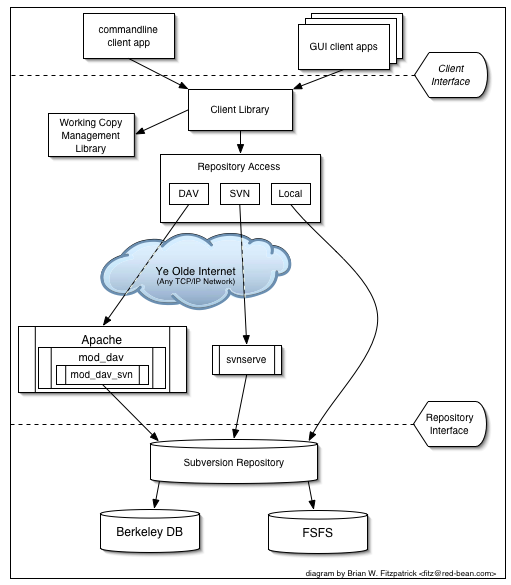
\includegraphics[scale=0.5]{subversion-diagram.png}}
 \caption{Subversion-Diagramm}
 \label{Subversion-Diagramm}	
\end{figure}
\end{center}
Das Diagramm erl�utert die Vorgehensweise des SVN in allen drei Schichten (User-Schicht, SVN-Schicht und Repository-Schicht). �ber eine Applikation oder �ber die Kommandozeile gibt der User seine Interaktion an. Daraufhin greift SVN mittels des Befehls auf das Repository zu (�ber DAV, SVN oder lokal) und f�hrt den Befehl auf dem Repository aus. Je nach Befehl werden Dateien hochgeladen, runtergeladen, hinzugef�gt, gel�scht, gemerged etc.\\
SVN bietet zwei unterschiedliche Backends zur Verwaltung der Repositorys an. Das eine ist die \emph{Berkley-Datenbank} und das andere ist das \emph{fsfs-Backend}. In der folgenden Tabelle werden die Unterschiede und Gemeinsamkeiten aufgelistet:
\begin{center}
% use packages: array
\begin{tabular}[c]{|p{6cm}|p{6cm}|}
\hline
Berkley-Datenbank & fsfs-Backend \\ \hline 
Speichert das Repository in einer Datenbank & Speichert das Repository in einer einzigen Datei \\ \hline
Transaktionen werden in der Datenbank gespeichert & Transaktionen werden als Unterordner gespeichert \\ \hline
Die Gr��e und der Zugriff spielen keine Rolle & Die Gr��e ist kleiner und der Zugriff ist nicht unbegrenzt \\ \hline
Benutzt einen $O(n�)$-Algorithmus, um den kompletten Ordner zu �berschreiben & Benutzt einen O(n) -Algorithmus, um die Dateien an das Repository ranzuh�ngen \\ \hline
Auscheken des letzten Baumes ist schnell & Auschecken des letzten Baumes ist etwas langsamer \\ \hline
Beim Crash bleibt die DB unbrauchbar bis sie repariert wird & Beim Crash ist nicht das komplette Repository betroffen, sondern evtl. nur die Transaktion \\ \hline
Repository-Backup funktioniert zur Laufzeit & Repository-Backup funktioniert zur Laufzeit \\ \hline
Repository kann nicht auf andere OS kopiert werden & Repository kann auf andere OS portiert werden\\ \hline
\end{tabular}
\end{center}
\vspace{1cm} 

Im Gegensatz zu CVS bietet SVN einige Merkmale, die das Arbeiten sehr viel einfacher gestalten. In der folgenden Liste, sind die Vorteile gegen�ber CVS aufgelistet:
\begin{itemize}
 \item SVN versioniert oder revisioniert grunds�tzlich das gesamte Projektarchiv und damit jeweils die gesamte Verzeichnisstruktur, w�hrend CVS auf der unabh�ngigen Versionierung jedes einzelnen Inhalts beruht
 \item  Mit Subversion ist es m�glich, Dateien oder Verzeichnisse zu verschieben oder umzubenennen, ohne die Versionsgeschichte zu verlieren
 \item �nderungen ("commits") sind  in Subversion atomar, das hei�t, eine �nderung wird entweder ganz oder gar nicht ins Repository gespeichert. Verbindungsabbr�che und mehrere gleichzeitige "commits" k�nnen somit nicht zu inkonsistenten Zust�nden f�hren
\end{itemize}

\subsection{Organisation des SVN-Repositories}

Die \marginpar{Ordnerstruktur} Strukturierung der Ordner ist wohl das wesentliche Hauptmerkmal des SVN. SVN arbeitet mit der Idee der Kopie. Das bedeutet, man besitzt eine Hauptentwicklungslinie die den Stamm des kompletten Projektes bildet. Im Falle des Studienprojektes \glqq DecidR\grqq{} (vgl. Abbildung \ref{fig:ordner}) ist \texttt{trunk} der Hauptordner, indem das Hauptprojekt abgespeichert wird. Da es dabei sinnlos ist, alle Dateien nur in dem \texttt{trunk} Ordner zu legen, ist eine weitere Untergliederung sinnvoll. Es wurden die Ordner \texttt{docs}, \texttt{prototype}, \texttt{seminars} und \texttt{src} angelegt. 

Im Unterordner \texttt{docs} befinden sich alle Dokumente, die in diesem Projekt erstellt werden (Angebot, Anforderungsanalyse, Spezifikation, Entwurf, Test, Handbuch usw.). F�r jedes weitere Dokument wurde ein weiterer Unterordner angelegt, indem dann die kompletten Dateien abgelegt werden. 

Der Unterordner \texttt{prototype} dient zur Ablage der Dateien f�r den Prototypen. Auch dieser enth�lt Unterordner, die sich speziell auf das Subprojekt beziehen. 

Der Ordner \texttt{seminars} bietet den Teammitgliedern die M�glichkeit ihr eigenes Seminar per Versionskontrolle zu erstellen. Jedes Teammitglied besitzt einen eigenen Ordner, den er selber weiter gestalten kann, wie er m�chte. 

Und im Unterordner \texttt{src} wird der Hauptcode abgelegt, der w�hrend der Implementierungsphase ensteht. 

Zudem gibt es noch den Ordner \texttt{tags}. Dieser Ordner dient der Markierung von gewissen Versionsst�nden. Hier werden alle Versionen abgelegt, die als stabil erachtet werden oder als Review-Version dienen. Das bedeutet, falls der erste Prototyp lauff�hig ist, wird die Version dort abgelegt, damit die Entwickler zu einem sp�teren Zeitpunkt genau wissen, auf welche Version sie sich berufen m�ssen, falls sie etwas am fertigen Prototypen �ndern m�chten. 

Letztlich bleibt noch der Ordner \texttt{branch}. In diesem Ordner werden nach der Philosophie des SVN Kopien des Stammordners \texttt{trunk} angelegt, um, wenn evtl. n�tig, andere Entwicklungspfade einzuschlagen. Der Ordner ist somit ein Zweig der Hauptentwicklungslinie. Man kann dann andere Entwicklungpfade einschlagen, ohne die Hauptentwicklungslinie zu besch�digen. 

\begin{figure}[h]
 \centering
 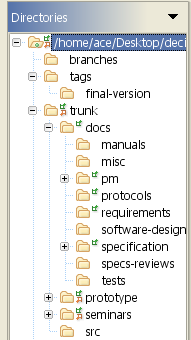
\includegraphics[scale=0.6]{ordertree.png}
 \caption{Ordnerstrukur des Studienprojektes \glqq DecidR\grqq{}}
  \label{fig:ordner}
\end{figure}

Diese Ordnerstruktur wird als Standard angesehen und von allen SVN Betreibern empfohlen. Letzten Endes bleibt es dem Versionsbeauftragtem �berlassen, wie er das SVN strukturiert. Der Versionsbeauftragte ist die Person im Projekt, die sich um die Ordnerstruktur im SVN k�mmert.

\subsection{Funktionsweise des SVN und Tools}

Im \marginpar{Funktionsweise des SVN} vorigen Unterkapitel wurde erl�utert, wie das SVN funktioniert. In diesem Unterkapitel wird erkl�rt was f�r Funktionalit�ten SVN bietet, bzw. wie man mit SVN arbeitet. Anschlie�end werden Tools f�r die Arbeit mit SVN aufgelistet. Bei den Befehlen bezieht sich die angegebene Adresse auf das SVN-Repository vom Studienprojekt \glqq DecidR\grqq.

Nachdem \marginpar{Befehle} das SVN-Repository auf einem Server angelegt und die Ordnerstruktur gew�hlt wurde, muss der Entwickler die gleiche Ordnerstruktur auf seinem Betriebssystem (OS) herstellen. Dazu bietet SVN einen Befehl an:
\begin{verbatim}
 svn checkout http://decidr.googlecode.com/svn/trunk/ decidr
\end{verbatim}
Dieser Befehl berechtigt den Entwickler nur das Lesen der Ordnerstruktur. Falls man selber Dateien hochladen oder �nderungen vornehmen m�chte, muss das Checkout verschl�sselt geschehen:
\begin{verbatim}
 svn checkout https://decidr.googlecode.com/svn/trunk/ 
 decidr --username username
\end{verbatim}
Man muss dabei seinen Benutzernamen und sein Passwort eingeben, erst dann erfolgt der Checkout in den Ordner, den man nach der Repository-Adresse angegeben hat. Beim ersten Checkout wird in dem Ordner eine \texttt{.svn} Datei erstellt, in der die kompletten Daten des SVN-Repositorys stehen.

S�mtliche Updates auf dem Repository kann man mit dem Update-Befehl auf sein OS holen:
\begin{verbatim}
 svn update decidr
\end{verbatim}
Dabei reicht es, wenn man den Ordner angibt der erneuert werden soll. Dieser muss aber die \texttt{.svn} Datei enthalten.

Falls man neue Dateien in das Repository laden m�chte, muss man zun�chst die Dateien vormerken. Dies geschieht mit:
\begin{verbatim}
 svn add file
\end{verbatim}
Daraufhin muss dem Repository noch mitgeteilt werden, dass die markierten Dateien nun hochgeladen und ins Repository aufgenommen werden sollen:
\begin{verbatim}
 svn commit decidr
\end{verbatim}
Beim commit ist es �blich, dass man noch Kommentare mitschreibt, zum besseren Verst�ndnis der �nderungen. Das realisiert man mit dem Parameter -m \glqq kommentar\grqq.

Um Konflikte zu vermeiden, falls zwei Entwickler gleichzeitig an einer Datei arbeiten, kann man mit Hilfe von SVN Dateien sperren lassen:
\begin{verbatim}
 svn lock filename
\end{verbatim}
Diese m�ssen nach Beenden der �nderung wieder entsperrt werden:
\begin{verbatim}
 svn unlock filename
\end{verbatim}


\subsection{Tools f�r SVN}

F�r \marginpar{Tools} SVN gibt es eine Reihe von Tools. Hier werden welche f�r MacOS, Windows, Linux und plattformunabh�ngige Systeme vorgestellt.
Plattformunabh�ngige Tools sind Tools, die auf jeder Plattform benutzt werden k�nnen. Im Studienprojekt benutzen wir das plattformunabh�ngige Tool smartSVN. Wir haben dieses Tool ausgew�hlt, damit wir ein einheitliches Tool besitzen, da unsere Teammitglieder mit Windows, Linux und MacOS arbeiten. 

Hier einige plattformunabh�ngige Tools:
\begin{itemize}
 \item rapidSVN \cite{rapidSVN}
 \item subcommander \cite{subcommander}
 \item smartSVN \cite{smartsvn}
\end{itemize}

Ein Tool f�r Windows, welches nicht auf einer Applikation beruht, sondern in Form des Contextmen�s alle Funktionen verf�gbar macht:
\begin{itemize}
 \item TortoiseSVN \cite{tortoiseSVN} 
\end{itemize}

Ein Tool f�r MacOS:
\begin{itemize}
 \item versions \cite{versions} 
\end{itemize}

Ein Tool f�r Eclipse, welches wir benutzen, um den Source-Code direkt in Eclipse auschecken, bzw. updaten und committen zu k�nnen:
\begin{itemize}
 \item subclipse \cite{subclipse} 
\end{itemize}





\section{Maven}
Maven kommt aus dem J�dischen (\emph{meyvn}) bzw. aus dem Hebr�ischem (\emph{mevin}) und bedeutet soviel wie Experte. Die genaue englische �bersetzung lautet accumulator of knowledge, quasi ein Speicher f�r Wissen. \\
Maven wurde als Ansatz im \emph{Apache Jakarta Turbine Project} \footnote{Turbine ist ein Servlet basiertes Framework f�r erfahrene Java-Entwickler, um schnell Web-Applikationen zu erstellen}  benutzt, um den Build-Prozess zu vereinfachen. Es gab einige verschiedene Projekte mit ihren eigenen Ant-Buildfiles, die alle unterschiedlich waren und die Jar-Dateien wurden alle ins CVS geladen.\\
Daraus resultierte der Wunsch eines einheitlichen automatisierten Verfahrens, um den kompletten Build-Prozess zu standardisieren. Dabei setzt sich Maven mit folgenden Zielen auseinander:
\begin{itemize}
 \item Vereinfachung des Build-Prozesses
 \item Bereitstellung eines einheitlichen Build-Systems
 \item Bereitstellung von Qualit�tsinformationen bez�glich des Projektes
 \item Bereitstellung von Richtlininen zur besten Entwicklung
 \item Transparente Migration von neuen Features (Pklug-In)\\
\end{itemize}
Au�erdem versucht Maven das Prinzip \emph{Convention over Configuration}\footnote{Das Ziel ist, die Zahl der Entscheidungen, die ein Entwickler trifft, zu verringern und dabei Einfachheit zu erreichen, ohne die Felxibilt�t zu beeinflussen} f�r den gesamten Software-Lebenszyklus zu verfolgen. \\
Die erste Version von Maven war noch stark an Ant angelehnt, sodass sich diese beiden Build-Methoden �hnelten. Die zweite Version verfolgte grundlegende neue Ans�tze und ist nicht mehr mit der vorherigen Version kompatibel.\\

\subsection{Die Philosophie Mavens}
\marginpar{pom.xml}Beim Erstellen eins Maven Projektes wird ein einheitliches Projektverzeichnis und eine einheitliche Projektstruktur verwendet. Maven erstellt eine XML-Datei, die sogenannte \emph{pom.xml}. In dieser stehen die Grunddaten f�r das Projekt. Zum Beispiel stehen in der Datei, der Name des Projektes, die Version, die Art des Paketes, das sp�ter erstellt werden soll, die URL, die sich auf das Projekt bezieht und die Abh�ngigkeiten, die das Projekt mit sich bringt und aufgel�st werden sollen, wenn das Projekt erstellt wird. \\
\marginpar{settings.xml}Zus�tzlich wird eine weitere Konfigurationsverwaltung erstellt, die \emph{settings.xml}. In ihr werden die Zugangsdaten f�r den Repository-Server und Deploy-Server gespeichert. Desweiteren werden die Einbindung von Plugins- oder Bibliotheken-Repositorys oder projekt�bergreifende Parameter eingestellt. Sowohl in der settings.xml als auch in der pom.xml gibt es sogennante Profile, die ein weiterer Mechanismus zur �nderung der Einstellungen sind. In ihr k�nnen abweichende Parameter gesetzt werden, wie z.B. f�r Filterdateien oder Repositorys.\\
\marginpar{.m2-Ordner}Wie schon erw�hnt werden bei der ersten Verwendung diese beiden XML-Dateien erstellt. Zus�tzlich wird noch ein weiterer Ordner erstellt. Dieser hei�t .m2 Ordner und in ihm befindet sich das lokale Repository, welches mit den Dateien des entfernten Maven-Repositorys gef�llt wird. Somit ist gew�hrleistet, dass bei einem erneuten Nutzen von Maven nicht alles aus dem entfernten Repository runtergeladen wird, sondern Maven greift nur noch auf das lokale zu, sofern die ben�tigten Pakete dort schon vorhanden sind. Wenn nicht, werden diese automatisch runtergeladen.\\
\marginpar{Zentrales Repository}Ein weiterer Grundgedanke besteht darin, s�mtliche Bibliotheken und Plugins an einem zentralen Ort zu verwalten. Dies vereinfacht bei vielen Projekten den Verwaltungsaufwand. Diese zentrale Repository bietet die Apache Group an. Man kann auch eigene Repositorys erstellen, der Vorteil besteht darin, dass man keine Internetverbindung ben�tigt und eine firmen�bergreifende Bibliothek erstellen kann. Der Vorteil des zentralen Repositorys liegt darin, dass Abh�ngigkeiten bereits abgelegt sind, und nicht manuell mit eingebaut werden m�ssen.\\
\marginpar{IDE} Es gibt f�r Eclipse und NetBeans Plugins, um Maven in den IDEs zu integrieren und dort auch zu nutzen. \\
Man sieht also, dass mit wenigen Konfigurationseinstellungen der Maven-Prozess ver�ndert werden kann. Aber diese Einstellungen �ndern nichts am automatisierten Vorgehen von Maven, dieser bleibt immer gleich. Das ist ein gro�er Vorteil. Den Maven baut seine Projekte durch das Project Object Model (POM) und somit ist ein einheitliches Build-System gew�hrleistet, was es wiederrum m�glich macht alle Maven Projekte zu verstehen. Dadurch spart man Zeit bei der Einarbeitung von anderen Projekten, da man die Bauweise kennt.\\
Maven basiert auf einer Plugin-Architektur, die es erlaubt verschiedene Plungins f�r verschiedene Anwendungen auf das Projekt anzuwenden, ohne diese explizit installieren zu m�ssen. Daher ist die Migration von Features sehr einfach gehalten und einfach m�glich. \\
\marginpar{Was Maven nicht ist!}Zum Schluss noch einige Dinge dar�ber was Maven nicht ist. Maven ist keine Erweiterung des Build-Tools Ant und ebenfalls nicht nur ausschlie�lich ein Dokumentations-Tool. Maven stellt die besten M�glichkeiten zur Verf�gung. Es kann durchaus sein, dass es manchmal nicht m�glich ist mit Maven ein Projekt zu bauen, weil die Struktur des Projektes so exotisch ist, dass eine Standardisierung gar nicht m�glich ist. Dann sollte man ,in diesem Fall, Maven lieber aufgeben und versuchen das Projekt auf eine andere Weise zu builden. \\
Beim kompletten Build-Prozess durchl�uft Maven verschiedene Phasen, in denen jeweils ein bestimmter Teil des Software-Lebenszyklus durchgearbeitet wird. Diese werden im n�chsten Abschnitt beschrieben.

\subsection{Die Phasen Mavens}
\begin{center}
% use packages: array
\begin{tabular}[!t]{|p{6cm}|p{6cm}|}\hline
 Validierungsphase & Hier wird die pom.xml auf ihre Struktur �berpr�ft, ob diese korrekt ist. Erst wenn die korrekt ist, kann der Prozess weitergef�hrt werden \\ \hline
 Kompilierungsphase & Hier wird das Projekt kompiliert. Beim ersten Kompilieren, werden alle n�tigen Plugins heruntergeladen. Danach greift Maven auf das lokale System zu, falls es Plugins ben�tigt und sucht dort nach ihnen. Maven kompiliert die Klassen, die im Standard-Verzeichnis liegen. Die werden dort beim Erstellen des Projektes hineingelegt. \\ \hline
 Testphase & Hier werden die generierten Testklassen kompiliert und ausgef�hrt. Dabei werden zus�tzliche Plugins f�r das Kompilieren der Testklassen heruntergeladen. Bevor die Testklassen ausgef�hrt werden, wird der Maincode kompiliert. \\ \hline
 Paketierungsphase & In dieser Phase wird eine jar-Datei erstellt. In der pom.xml kann man angeben, was in dieser Phase erstellt werden soll. Die jar-Datei wird in einem standardisiertem Verzeichnis abgelegt. \\ \hline
 Integrations-Test & Hier wird durch ein Plugin das fertig Paket in eine Umgebung integriert und getestet. \\ \hline
 Verifizierungsphase & Hier wird das Paket �berpr�ft, ob es bestimmte Dateien/Ordner erh�lt und pr�ft den Inhalt auf ihre Struktur. \\ \hline
 Installationsphase & In dieser Phase wird das Paket, das im lokalen Maven-Repository liegt, installiert. \\ \hline
 Deployment & Ein Plugin f�r Maven sorgt daf�r, dass das erstellte Paket auf einem entfernten Repository gelegt wird, sodass andere Entwickler das Paket nutzen k�nnen. Alle n�tigen Informationen werden aus der pom.xml entnommen, sodass ein problemloses Deployment stattfinden kann. \\ \hline
 Site & Nun wird eine Seite erstellt, mit allen Informationen bez�glich des Projektes, sodass alle Informationen an einem Punkt sind. \\ \hline
 Clean & Clean l�scht den Zielordner mit all seinen Builddaten. \\ \hline
\end{tabular}
\end{center}

\subsection{Vergleich mvn, make und ant}
Maven ist das zweite Buildprojekt von Apache. Das erste Buildprojekt war \emph{ant}. Ant ist wohl das heutzutage weit verbreiteste Build-Tool. Es existiert noch ein weiteres Build-Tool und zwar \emph{make}. \emph{Make} ist Teil des POSIX-Standards, dessen gegenw�rtige Bezeichnung IEEE Std 1003.1, 2004 Edition lautet.\\
\marginpar{Apache-Ant}Apache Ant ist ein Java-basiertes Werkzeugt zur automatischen Erzeugung von Programmen aus Quelltext. Ant ist ein Akronym und steht f�r Another Neat Tool. Es wurde 1999 von James Duncan Davidson entwickelt, der ein Werkzeug wie make nur f�r Java ben�tigte. Ant wird durch eine einzige XML-Datei gesteuert, der sogenannten \emph{build.xml}. In dieser Build-Datei wird ein Project ermittelt, welches das Wurzelelement darstellt. Desweiteren besitzt die build.xml sogenannte \emph{Targets}. Diese sind vergleichbar mit Funktionen in Programmiersprachen und k�nnen von au�en �ber die Kommandozeile aufgerufen werden. Abh�ngigkeiten, die in den Targets definiert werden, l�st Ant auf und dient zum Bauen des Programmes. Da es sich um eine XML-Datei handelt ist diese nicht von Tabulatorzeichen oder sonstiges abh�ngig. Dies ist eine Verbesserung gegen�ber dem alten Build-Tool make. \\
\marginpar{make}Make liest ein sogenanntes \emph{Makefile}, in dem der �bersetzungsprozess von Programmen formalisiert erfasst ist. Diese Formalisierung beschreibt, welche Quelltextdateien der Compiler zu welchen Objektdateien verarbeitet, und welche Objektdateien vom Linker dann zu Programmbibliotheken oder ausf�hrbaren Programmen verbunden werden. Alle Schritte erfolgen unter Beachtung der Abh�ngigkeiten, die m�glicherweise durch die Dateiorganisation gegeben sein k�nnen. Bei der Abarbeitung wird eine Umwandlung von einer Quelldatei nur dann vorgenommen, wenn die Quelldatei neuer als die Objektdatei ist. Der Vorteil dabei ist, dass bei kleinen Ver�nderungen in gro�en Projekten nicht die komplette Kompilation durchgef�hrt werden muss. Jedoch m�ssen alle Abh�ngigkeiten in der Makefile beschrieben werden, was bei sehr gro�en Projekten nicht immer leicht zu realisieren ist.\\
\marginpar{Vor- und Nachteile von mvn, ant und make}Der klare Vorteil bei Ant und Make ist die Vielzahl an Literatur, die es mittlerweile gibt und die praktische Erfahrung, da diese beiden Build-Tools am weitesten verbreitet sind. Au�erdem ist die Einarbeitung in Ant einfacher und es ist auch leichter zu handhaben. Die Einarbeitung in Maven f�llt wesentlicher gr��er aus. Daf�r bietet Maven eine einheitliche Projektstruktur und eine zentrale Verwaltung von Bibliotheken durch das Repository. Zudem ist es leicht erweiterbar, was f�r ant und make nicht gilt. Bei make spielen die Abh�ngigkeiten eine gro�e Rolle und k�nnen bei gro�en Projekten zu Problemen f�hren, um die sich Maven bei seinen Projekten nicht k�mmern muss. Einen weiteren Zusatz bietet das site von Maven, in der Informationen zum Projekt bereitgestellt werden. Maven und ant sind XML-basiert im Gegensatz zu make, welches einem Shellskript �hnelt.

\subsection{Hudson continuous integration}
Hudson contiuous integration ist ein erweiterbares, webbasiertes Tool zur kontinuierlichen Integration in agilen Softwareprojekten. Kontinuierliche Integration bedeutet eine fortlaufende, permanente Integration der den Prozess des vollst�ndigen Neubildens und Testens einer Anwendung beschreibt. Dabei spielt das agile Softwareprojekt eine bedeutende Rolle. Denn durch die Agilit�t der Software wird die permanente Integration m�glich. Das Extreme Programming ist ein Beispiel f�r solch ein agiles Softwareprojekt. Sobald �nderungen in der Anwendung vorgenommen werden, wird die komplette Anwendung neu gebaut und automatisch getestet. Falls dieser Test erfolgreich ist, wird die Anwendung in die n�chste Stufe gereicht, falls nicht, findet ein Rollback statt und die Entwickler werden aufgefordert die Anwendung zu verbessern. Und genau das �bernimmt Hudson, in automatisierter Form. \\
\marginpar{Funktionalit�ten}Hudson wurde in erster Linie von Kohsuke Kawaguchi, Mitarbeiter von Sun Microsystems, entwickelt. Bis auf die Icons steht das komplette Programm unter der MIT-Lizenz. Hudson ist in Java geschrieben und l�uft auf einem beliebigen Servlet-Container. Es werden s�mtliche g�ngigen Build-Tools verwendet, wie Apache-Ant oder Apache-Maven. Zus�tzlich bietet Hudson noch die M�glichkeit der Versionsverwaltung (CVS oder Subversion). Desweiteren bietet Hudson die M�glichkeit �nderungen per Email zu verschicken und so die betreffenden Entwickler zu informieren. \\
\marginpar{Vorteile}Dabei steht die Einfachheit an erster Stelle. Gerade in Bezug auf Maven bietet Hudson eine sehr einfache und praktikable M�glichkeit. Es ist m�glich ein Maven Projekt zu erstellen, sodass Hudson es �berwacht und �nderungen zur sofortigen Neubildung und Testen der Anwendung f�hrt. Durch die kontinuierliche Integration, die Hudson bietet, wird die Programmierung vorteilhafter. Dabei werden
\begin{itemize}
 \item Fehler laufend entdeckt und behoben und nicht erst vor dem Meilenstein
 \item fr�he Warnungen bei nicht passenden Bestandteilen ausgegeben
 \item Fehler bei Unit-Tests sofort entdeckt
 \item lauff�hige Versionen f�r Test-, Demo- und Vertriebszwecke angeboten
 \item die Entwickler gezwungen verwantwortungsvoller mit ihren T�tigkeiten umzugehen, um Fehler zu vermeiden
\end{itemize}

\section{Zusammenfassung}
Im der Ausarbeitung habe ich zwei g�ngige Tools beschrieben, die heutzutage als Standard gelten, wenn man gr��ere Projekte entwickeln m�chte.\\
Subversion ist nicht mehr vom Projektmanagement weg zu denken. Es bietet eine stabile Grundlage zur Sicherung der Dateien und zur Verwaltung der Dateien, sodass eine gro�e Softwaregruppe mit bis zu zehn Entwicklern gleichzeitig an einem Projekt arbeiten kann, ohne dass es zu Konflikten kommt. Und durch das ausgepr�gte Loggen kann man immer nachvollziehen, welche �nderunge vorgenommen wurden. Zum anderen dient Subversion ebenfalls als Nachweis. Durch weitere Programme kann man sich die kompletten svn-Daten auflisten lassen und kann �berpr�fen, welcher Entwickler wieviel hochgeladen hat. Die m�ssen nicht ausschlaggebend f�r eine Bewertung des Entwicklers sein, aber man kann sie in die Bewertung mit einbeziehen. Man sieht also, dass Subversion mehr zu bieten hat als nur eine Versionsverwaltung. \\
Maven erleichtert einige Aufgaben eines Entwicklers oder einer Entwicklergruppe. Der standardisierte Software-Lebenszyklus wird automatisiert und unterschiedliche Strukturen werden aufgehoben, sodass eine einheitliche Anwendung entsteht, die sp�ter ohne gro�e Probleme in anderen Projekten integriert werden kann. Dabei werden fr�hzeitig Fehler entdeckt, die Entwickler vor gro�en Problemen stellen k�nnten. In Kombination mit Hudson, der permanent bei neuen �nderungen die Anwendung neu baut und testet, ist Maven ein weiteres Tool f�r das Projektmanagement, mit dem Entwickler sehr viel Zeit sparen k�nnen und diese Zeit in Phasen investieren k�nnen, die der Planung des Projektes dienen (Projektplan, Spezifikation, Entwurf). Das gew�hrleistet eine bessere Planung mit hoher Qualit�t, wenigen Fehlern und einer stabilen Software. \\
In Bezug auf das Studienprojekt \flqq DecidR \frqq wird Subversion schon benutzt. Ob sich Maven und Hudson mitintegrieren lassen wird sich entscheiden. Meine pers�nlicher Wunsch w�re es, diese Tools zu benutzen.

\bibliographystyle{splncs}
\bibliography{Seminar}

Alle URLs wurden zuletzt am \today{} gepr�ft.

\end{document}
